\documentclass{article}\usepackage[]{graphicx}\usepackage[]{xcolor}
% maxwidth is the original width if it is less than linewidth
% otherwise use linewidth (to make sure the graphics do not exceed the margin)
\makeatletter
\def\maxwidth{ %
  \ifdim\Gin@nat@width>\linewidth
    \linewidth
  \else
    \Gin@nat@width
  \fi
}
\makeatother

\definecolor{fgcolor}{rgb}{0.345, 0.345, 0.345}
\newcommand{\hlnum}[1]{\textcolor[rgb]{0.686,0.059,0.569}{#1}}%
\newcommand{\hlstr}[1]{\textcolor[rgb]{0.192,0.494,0.8}{#1}}%
\newcommand{\hlcom}[1]{\textcolor[rgb]{0.678,0.584,0.686}{\textit{#1}}}%
\newcommand{\hlopt}[1]{\textcolor[rgb]{0,0,0}{#1}}%
\newcommand{\hlstd}[1]{\textcolor[rgb]{0.345,0.345,0.345}{#1}}%
\newcommand{\hlkwa}[1]{\textcolor[rgb]{0.161,0.373,0.58}{\textbf{#1}}}%
\newcommand{\hlkwb}[1]{\textcolor[rgb]{0.69,0.353,0.396}{#1}}%
\newcommand{\hlkwc}[1]{\textcolor[rgb]{0.333,0.667,0.333}{#1}}%
\newcommand{\hlkwd}[1]{\textcolor[rgb]{0.737,0.353,0.396}{\textbf{#1}}}%
\let\hlipl\hlkwb

\usepackage{framed}
\makeatletter
\newenvironment{kframe}{%
 \def\at@end@of@kframe{}%
 \ifinner\ifhmode%
  \def\at@end@of@kframe{\end{minipage}}%
  \begin{minipage}{\columnwidth}%
 \fi\fi%
 \def\FrameCommand##1{\hskip\@totalleftmargin \hskip-\fboxsep
 \colorbox{shadecolor}{##1}\hskip-\fboxsep
     % There is no \\@totalrightmargin, so:
     \hskip-\linewidth \hskip-\@totalleftmargin \hskip\columnwidth}%
 \MakeFramed {\advance\hsize-\width
   \@totalleftmargin\z@ \linewidth\hsize
   \@setminipage}}%
 {\par\unskip\endMakeFramed%
 \at@end@of@kframe}
\makeatother

\definecolor{shadecolor}{rgb}{.97, .97, .97}
\definecolor{messagecolor}{rgb}{0, 0, 0}
\definecolor{warningcolor}{rgb}{1, 0, 1}
\definecolor{errorcolor}{rgb}{1, 0, 0}
\newenvironment{knitrout}{}{} % an empty environment to be redefined in TeX

\usepackage{alltt}
\usepackage[sc]{mathpazo}
\renewcommand{\sfdefault}{lmss}
\renewcommand{\ttdefault}{lmtt}
\usepackage[T1]{fontenc}
\usepackage{geometry}
\geometry{verbose,tmargin=2.5cm,bmargin=2.5cm,lmargin=2.5cm,rmargin=2.5cm}
\setcounter{secnumdepth}{2}
\setcounter{tocdepth}{2}
\usepackage[unicode=true,pdfusetitle,
 bookmarks=true,bookmarksnumbered=true,bookmarksopen=true,bookmarksopenlevel=2,
 breaklinks=false,pdfborder={0 0 1},backref=false,colorlinks=false]
 {hyperref}
\hypersetup{
 pdfstartview={XYZ null null 1}}

\makeatletter
%%%%%%%%%%%%%%%%%%%%%%%%%%%%%% User specified LaTeX commands.
\renewcommand{\textfraction}{0.05}
\renewcommand{\topfraction}{0.8}
\renewcommand{\bottomfraction}{0.8}
\renewcommand{\floatpagefraction}{0.75}

\makeatother
\IfFileExists{upquote.sty}{\usepackage{upquote}}{}
\begin{document}



\title{\title{\title{\title{\title{\title{\title{\title{}}}}}}}}



\maketitle
The results below are generated from an R script.

\begin{knitrout}
\definecolor{shadecolor}{rgb}{0.969, 0.969, 0.969}\color{fgcolor}\begin{kframe}
\begin{alltt}
\hlcom{# Assignment: Week4 #1}
\hlcom{# Name: Couto, Maria}
\hlcom{# Date: 2023-06-30}

\hlkwd{setwd}\hlstd{(}\hlstr{"C:/Users/ait0s/OneDrive/Documents/GitHub/Couto_DSC520"}\hlstd{)}

\hlcom{# Load the `scores.csv' data set}

\hlstd{datasetforscores} \hlkwb{<-} \hlkwd{read.csv}\hlstd{(}\hlstr{"scores.csv"}\hlstd{)}
\hlstd{datasetforscores}
\end{alltt}
\begin{verbatim}
##    Count Score Section
## 1     10   200  Sports
## 2     10   205  Sports
## 3     20   235  Sports
## 4     10   240  Sports
## 5     10   250  Sports
## 6     10   265 Regular
## 7     10   275 Regular
## 8     30   285  Sports
## 9     10   295 Regular
## 10    10   300 Regular
## 11    20   300  Sports
## 12    10   305  Sports
## 13    10   305 Regular
## 14    10   310 Regular
## 15    10   310  Sports
## 16    20   320 Regular
## 17    10   305 Regular
## 18    10   315  Sports
## 19    20   320 Regular
## 20    10   325 Regular
## 21    10   325  Sports
## 22    20   330 Regular
## 23    10   330  Sports
## 24    30   335  Sports
## 25    10   335 Regular
## 26    20   340 Regular
## 27    10   340  Sports
## 28    30   350 Regular
## 29    20   360 Regular
## 30    10   360  Sports
## 31    20   365 Regular
## 32    20   365  Sports
## 33    10   370  Sports
## 34    10   370 Regular
## 35    20   375 Regular
## 36    10   375  Sports
## 37    20   380 Regular
## 38    10   395  Sports
\end{verbatim}
\begin{alltt}
\hlcom{# What are the observational units in this study?}

  \hlcom{# In statistics, observational units are the entities (people,things,etc.)}
  \hlcom{# and may sometimes be referred as subject if they are people.}
  \hlcom{# In a datafarame,}
  \hlcom{# however, every row is considered an observation and every column is a}
  \hlcom{# variable. There are 38 rows and 3 columns in this dataset}

\hlkwd{nrow}\hlstd{(datasetforscores)}
\end{alltt}
\begin{verbatim}
## [1] 38
\end{verbatim}
\begin{alltt}
\hlcom{# Identify the variables mentioned in the narrative paragraph }
\hlcom{#   and determine which are categorical and quantitative?}

  \hlcom{# Categorical Variables: sections (sports and variety)}
  \hlcom{# Quantitative: course grades and total points earned}

\hlcom{# Create one variable to hold a subset of your data set that contains }
\hlcom{#   only the Regular Section and one variable for the Sports Section.}

\hlkwd{library}\hlstd{(plyr)}
\hlkwd{library}\hlstd{(dplyr)}
\hlkwd{select}\hlstd{(datasetforscores,} \hlstr{"Section"}\hlstd{)}
\end{alltt}
\begin{verbatim}
##    Section
## 1   Sports
## 2   Sports
## 3   Sports
## 4   Sports
## 5   Sports
## 6  Regular
## 7  Regular
## 8   Sports
## 9  Regular
## 10 Regular
## 11  Sports
## 12  Sports
## 13 Regular
## 14 Regular
## 15  Sports
## 16 Regular
## 17 Regular
## 18  Sports
## 19 Regular
## 20 Regular
## 21  Sports
## 22 Regular
## 23  Sports
## 24  Sports
## 25 Regular
## 26 Regular
## 27  Sports
## 28 Regular
## 29 Regular
## 30  Sports
## 31 Regular
## 32  Sports
## 33  Sports
## 34 Regular
## 35 Regular
## 36  Sports
## 37 Regular
## 38  Sports
\end{verbatim}
\begin{alltt}
\hlstd{regular_section} \hlkwb{<-} \hlkwd{filter}\hlstd{(datasetforscores, Section} \hlopt{==} \hlstr{"Regular"}\hlstd{)}
\hlstd{sports_section} \hlkwb{<-} \hlkwd{filter}\hlstd{(datasetforscores, Section} \hlopt{==} \hlstr{"Sports"}\hlstd{)}
\hlstd{regular_section}
\end{alltt}
\begin{verbatim}
##    Count Score Section
## 1     10   265 Regular
## 2     10   275 Regular
## 3     10   295 Regular
## 4     10   300 Regular
## 5     10   305 Regular
## 6     10   310 Regular
## 7     20   320 Regular
## 8     10   305 Regular
## 9     20   320 Regular
## 10    10   325 Regular
## 11    20   330 Regular
## 12    10   335 Regular
## 13    20   340 Regular
## 14    30   350 Regular
## 15    20   360 Regular
## 16    20   365 Regular
## 17    10   370 Regular
## 18    20   375 Regular
## 19    20   380 Regular
\end{verbatim}
\begin{alltt}
\hlstd{sports_section}
\end{alltt}
\begin{verbatim}
##    Count Score Section
## 1     10   200  Sports
## 2     10   205  Sports
## 3     20   235  Sports
## 4     10   240  Sports
## 5     10   250  Sports
## 6     30   285  Sports
## 7     20   300  Sports
## 8     10   305  Sports
## 9     10   310  Sports
## 10    10   315  Sports
## 11    10   325  Sports
## 12    10   330  Sports
## 13    30   335  Sports
## 14    10   340  Sports
## 15    10   360  Sports
## 16    20   365  Sports
## 17    10   370  Sports
## 18    10   375  Sports
## 19    10   395  Sports
\end{verbatim}
\begin{alltt}
\hlcom{# Use the Plot function to plot each Sections scores and }
\hlcom{# the number of students achieving that score. }
\hlcom{# Use additional Plot Arguments to label the graph }
\hlcom{# and give each axis an appropriate label. }


\hlkwd{library}\hlstd{(ggplot2)}
\hlkwd{theme_set}\hlstd{(}\hlkwd{theme_minimal}\hlstd{())}

\hlcom{# Plot each Section (Regular Scatter & Histogram)}
\hlkwd{ggplot}\hlstd{(regular_section,} \hlkwd{aes}\hlstd{(Score, Count))} \hlopt{+}
  \hlkwd{geom_point}\hlstd{(}\hlkwc{colour} \hlstd{=} \hlstr{"green"}\hlstd{,}\hlkwc{size} \hlstd{=} \hlnum{3}\hlstd{)} \hlopt{+}
  \hlkwd{ggtitle}\hlstd{(}\hlstr{"Plot: Regular Section"}\hlstd{)}
\end{alltt}
\end{kframe}

{\centering 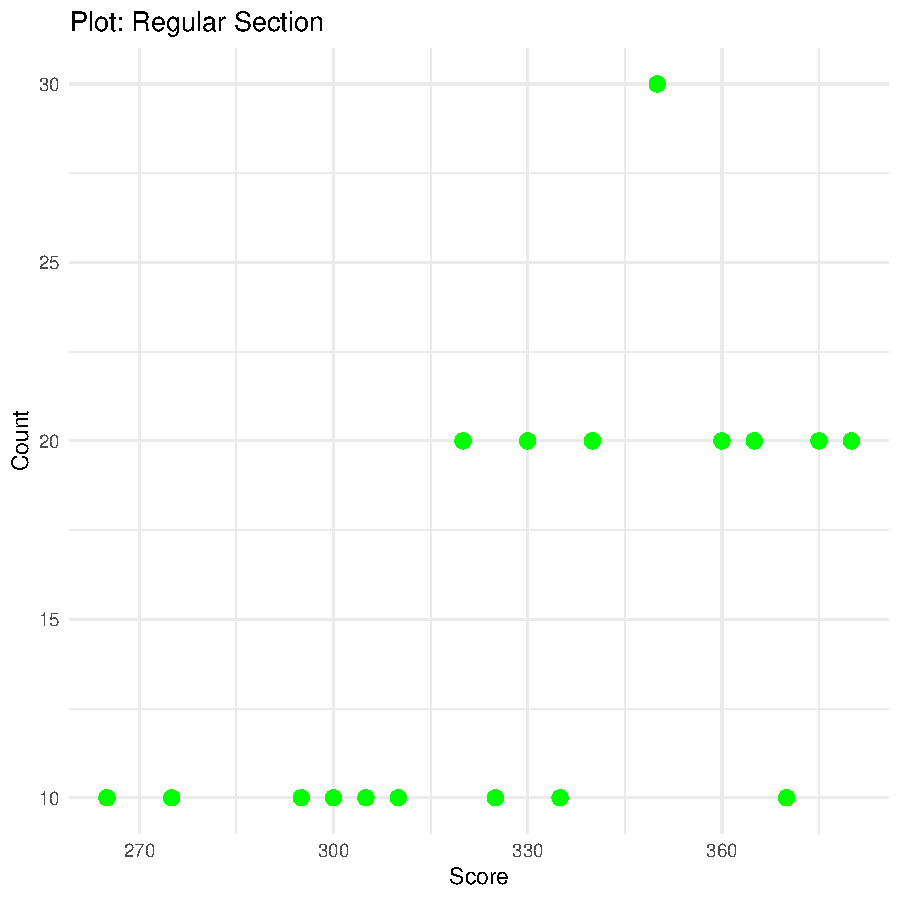
\includegraphics[width=.6\linewidth]{figure/week4-assignment-01-Couto-Maria-Rnwauto-report-1} 

}


\begin{kframe}\begin{alltt}
\hlkwd{ggplot}\hlstd{(regular_section,} \hlkwd{aes}\hlstd{(}\hlkwc{y}\hlstd{=Count,}\hlkwc{x}\hlstd{=Score))} \hlopt{+}
  \hlkwd{geom_bar}\hlstd{(}\hlkwc{position} \hlstd{=} \hlstr{'dodge'}\hlstd{,} \hlkwc{stat}\hlstd{=}\hlstr{'identity'}\hlstd{,}\hlkwc{colour}\hlstd{=}\hlstr{"black"}\hlstd{,}\hlkwc{fill}\hlstd{=}\hlstr{"green"}\hlstd{)} \hlopt{+}
  \hlkwd{ggtitle}\hlstd{(}\hlstr{"Bar: Regular Section"}\hlstd{)}
\end{alltt}
\end{kframe}

{\centering 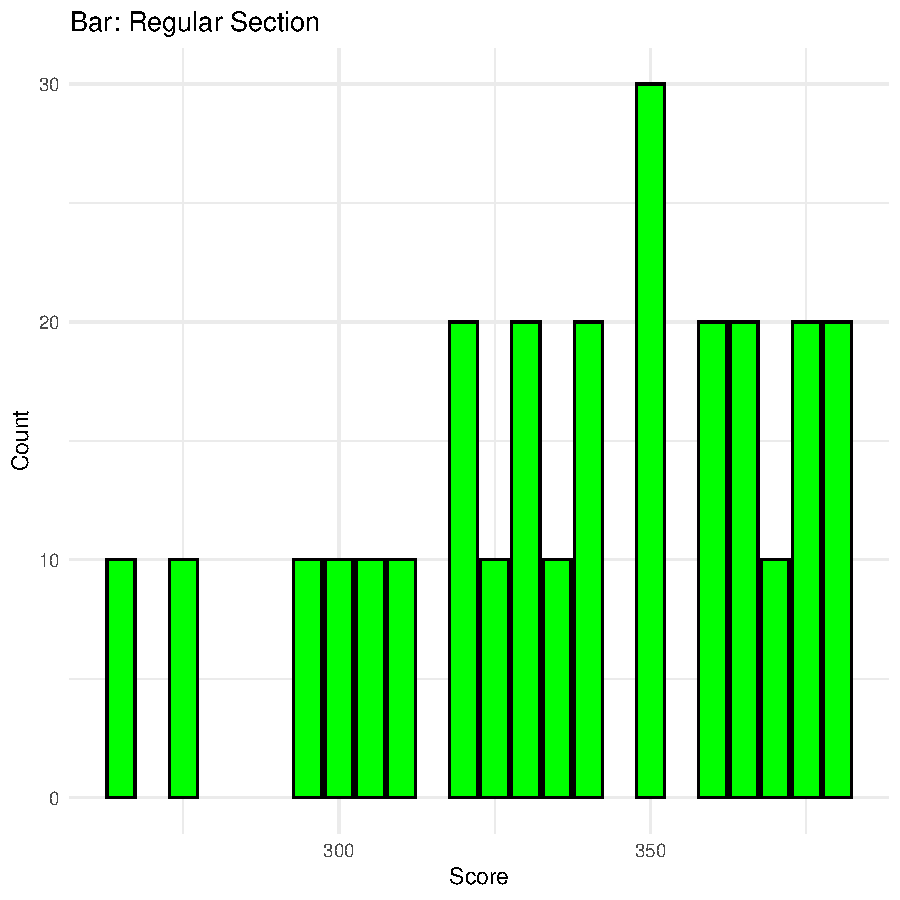
\includegraphics[width=.6\linewidth]{figure/week4-assignment-01-Couto-Maria-Rnwauto-report-2} 

}


\begin{kframe}\begin{alltt}
\hlcom{# Plot each Section (Sports Scatter & Histogram)}

\hlkwd{ggplot}\hlstd{(sports_section,} \hlkwd{aes}\hlstd{(Score, Count))} \hlopt{+}
  \hlkwd{geom_point}\hlstd{(}\hlkwc{colour} \hlstd{=} \hlstr{"blue"}\hlstd{,}\hlkwc{size} \hlstd{=} \hlnum{3}\hlstd{)} \hlopt{+}
  \hlkwd{ggtitle}\hlstd{(}\hlstr{"Plot: Sports Section"}\hlstd{)}
\end{alltt}
\end{kframe}

{\centering 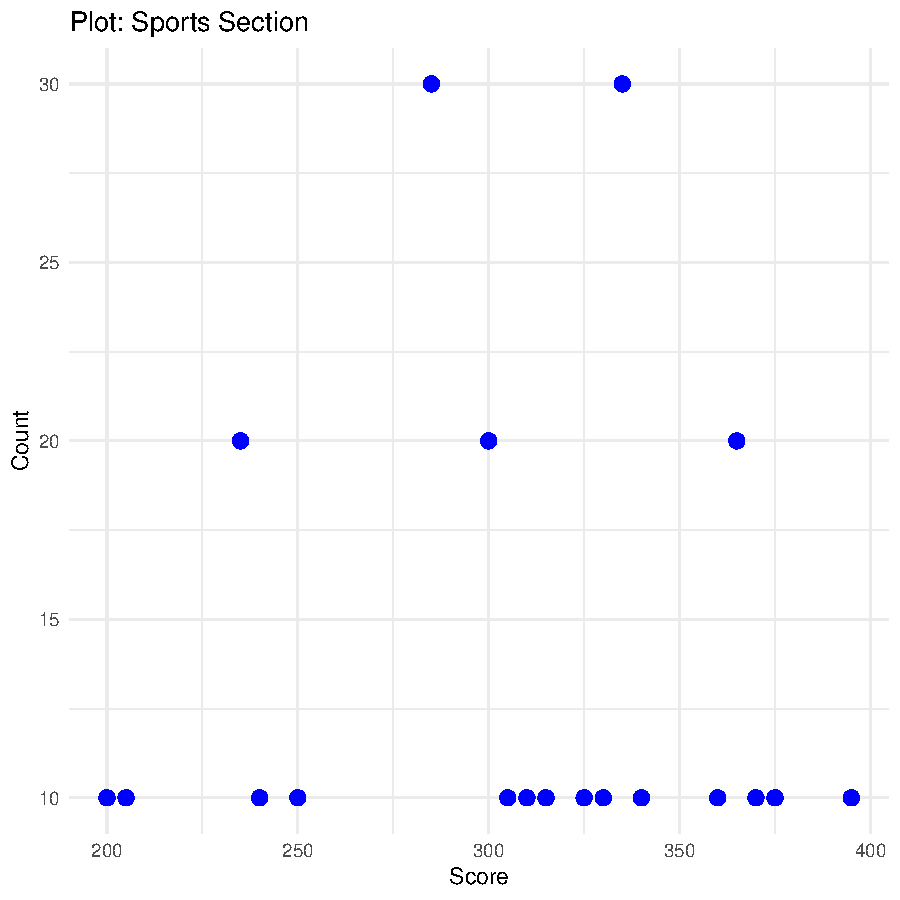
\includegraphics[width=.6\linewidth]{figure/week4-assignment-01-Couto-Maria-Rnwauto-report-3} 

}


\begin{kframe}\begin{alltt}
\hlkwd{ggplot}\hlstd{(sports_section,} \hlkwd{aes}\hlstd{(}\hlkwc{y}\hlstd{=Count,}\hlkwc{x}\hlstd{=Score))} \hlopt{+}
  \hlkwd{geom_bar}\hlstd{(}\hlkwc{position} \hlstd{=} \hlstr{'dodge'}\hlstd{,} \hlkwc{stat}\hlstd{=}\hlstr{'identity'}\hlstd{,}\hlkwc{colour}\hlstd{=}\hlstr{"black"}\hlstd{,}\hlkwc{fill}\hlstd{=}\hlstr{"blue"}\hlstd{)} \hlopt{+}
  \hlkwd{ggtitle}\hlstd{(}\hlstr{"Bar: Sports Section"}\hlstd{)}
\end{alltt}
\end{kframe}

{\centering 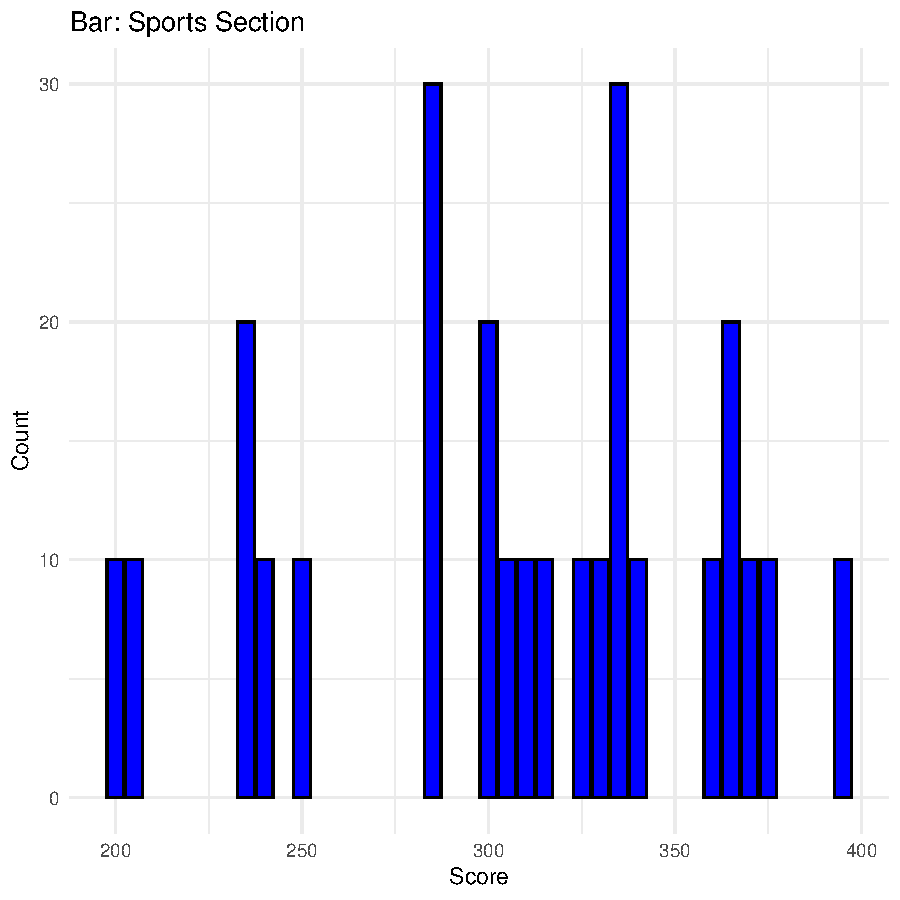
\includegraphics[width=.6\linewidth]{figure/week4-assignment-01-Couto-Maria-Rnwauto-report-4} 

}


\begin{kframe}\begin{alltt}
\hlcom{# Comparing and contrasting the point distributions between the two section, }
\hlcom{# looking at both tendency and consistency: Can you say that one section tended }
\hlcom{# to score more points than the other? Justify and explain your answer.}
  \hlcom{# we can see that the regular section has a tendency to score more.}
  \hlcom{# the bar chart for the regular section is unimodal with one peak and}
  \hlcom{# has a distribution that is left -skewed. Meaning, more participants}
  \hlcom{# scored higher and the lower tail is longer on the left side.}
  \hlcom{# The sports section,on the other hand, has a bimodal distribution with two }
  \hlcom{# distinct peaks and has multiple modes where different values}
  \hlcom{# appear more in the dataset. }


\hlcom{# Did every student in one section score more points than every student }
\hlcom{# in the other section? If not, explain what a statistical tendency means }
\hlcom{# in this context.}
\hlcom{# For this question, I plotted the values of both sections side by side}
\hlcom{# to show the comparison between the two. The visuals show us}
\hlcom{# that the sports section has both the highest and the lowest score}
\hlcom{# in the dataset. So not every student in one section score more}
\hlcom{# point than the other. Rather, the scores are more distributed}
\hlcom{# between the two sections. Statistical tendency helps us}
\hlcom{# describe a dataset by showing the frequency of the distribution of the}
\hlcom{# observations. The charts help us see the mode or the frequency of the}
\hlcom{# occurence in each data points. The graph shows that in the regular section,}
\hlcom{# the data points gravitate toward the higher end of the x axis which is a good}
\hlcom{# indicator that the regular section, overall, scored higher points than the }
\hlcom{# sports section.}

\hlcom{#Side-by_Side Plot comparison for Regular and Sports Section}

\hlkwd{ggplot}\hlstd{(datasetforscores,} \hlkwd{aes}\hlstd{(}\hlkwc{x}\hlstd{=Score,}\hlkwc{y}\hlstd{=Count,}\hlkwc{colour}\hlstd{=Section))} \hlopt{+}
  \hlkwd{geom_point}\hlstd{(}\hlkwc{size} \hlstd{=} \hlnum{2}\hlstd{)} \hlopt{+}
  \hlkwd{scale_color_manual}\hlstd{(}\hlkwc{values} \hlstd{=} \hlkwd{c}\hlstd{(}\hlstr{"Regular"}\hlstd{=}\hlstr{"green"}\hlstd{,}\hlstr{"Sports"}\hlstd{=}\hlstr{"blue"}\hlstd{))}
\end{alltt}
\end{kframe}

{\centering 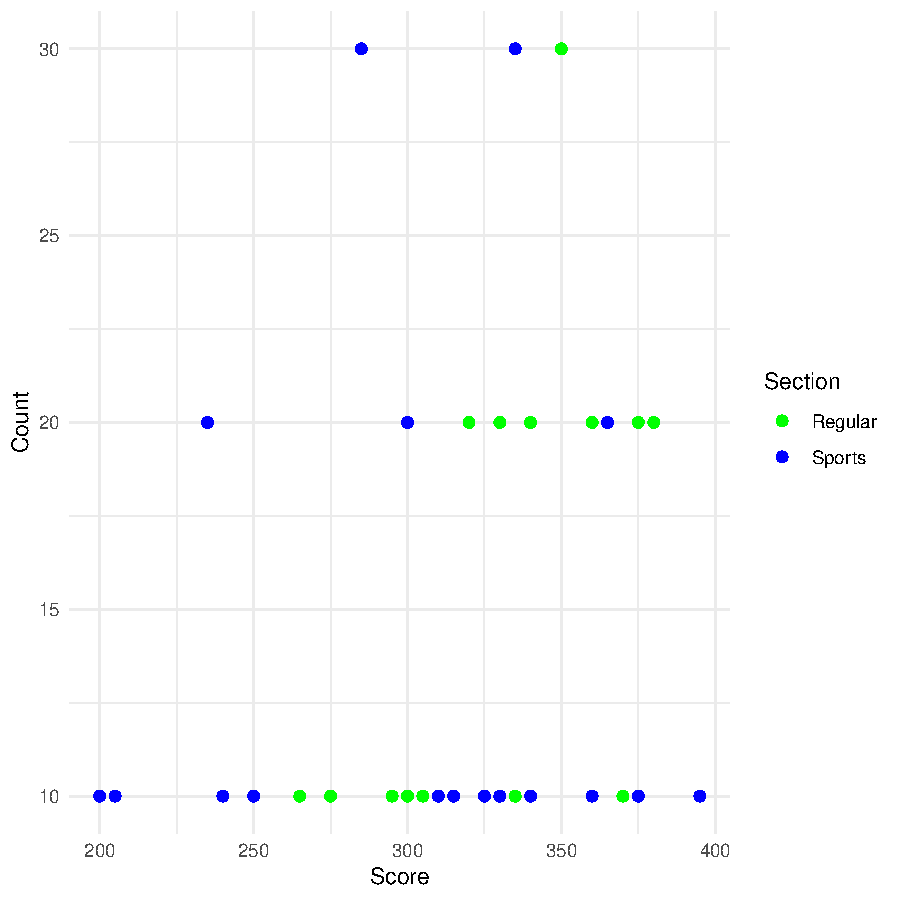
\includegraphics[width=.6\linewidth]{figure/week4-assignment-01-Couto-Maria-Rnwauto-report-5} 

}


\begin{kframe}\begin{alltt}
\hlcom{#Side-by_Side Bar comparison for Regular and Sports Section}


\hlkwd{ggplot}\hlstd{(datasetforscores,} \hlkwd{aes}\hlstd{(}\hlkwc{fill}\hlstd{=Section,}\hlkwc{y}\hlstd{=Count,}\hlkwc{x}\hlstd{=Score))} \hlopt{+}
  \hlkwd{geom_bar}\hlstd{(}\hlkwc{position} \hlstd{=} \hlstr{'dodge'}\hlstd{,} \hlkwc{stat}\hlstd{=}\hlstr{'identity'}\hlstd{)}
\end{alltt}
\end{kframe}

{\centering 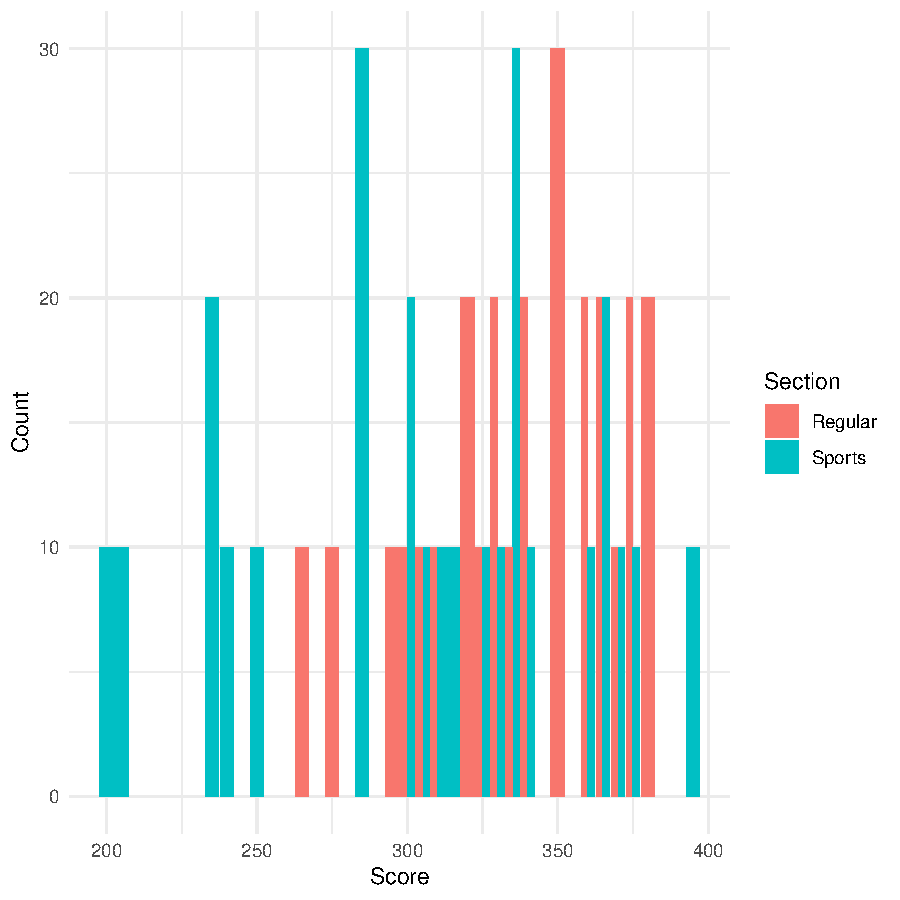
\includegraphics[width=.6\linewidth]{figure/week4-assignment-01-Couto-Maria-Rnwauto-report-6} 

}


\begin{kframe}\begin{alltt}
\hlcom{# What could be one additional variable that was not mentioned }
\hlcom{# in the narrative that could be influencing the point distributions }
\hlcom{# between the two sections}
\hlcom{# On the narrative- it speaks to  course grades and total points }
\hlcom{# earned in the course as the quantitative value. However, the columns}
\hlcom{# in the dataset shows counts, scores, and section. I'm assuming then, }
\hlcom{# that the count refers to the number of students who achieved the score}
\hlcom{# and their respective sections for each row. For example, does}
\hlcom{# gender play a role on whether or not a student would choose}
\hlcom{# to go to a course exclusive to sports application? While there are a lot of}
\hlcom{# variables that could affect the score, I would also be interested in }
\hlcom{# seeing the grades if the students prior to the professor teaching}
\hlcom{# the section. This would tell us if students who tend to perform better}
\hlcom{# has a tendency to enroll in the sports section or would they prefer to be}
\hlcom{# given a variety of application areas when they are learning their}
\hlcom{# lesson. }
\end{alltt}
\end{kframe}
\end{knitrout}

The R session information (including the OS info, R version and all
packages used):

\begin{knitrout}
\definecolor{shadecolor}{rgb}{0.969, 0.969, 0.969}\color{fgcolor}\begin{kframe}
\begin{alltt}
\hlkwd{sessionInfo}\hlstd{()}
\end{alltt}
\begin{verbatim}
## R version 4.3.0 (2023-04-21 ucrt)
## Platform: x86_64-w64-mingw32/x64 (64-bit)
## Running under: Windows 11 x64 (build 22621)
## 
## Matrix products: default
## 
## 
## locale:
## [1] LC_COLLATE=English_United States.utf8  LC_CTYPE=English_United States.utf8   
## [3] LC_MONETARY=English_United States.utf8 LC_NUMERIC=C                          
## [5] LC_TIME=English_United States.utf8    
## 
## time zone: America/New_York
## tzcode source: internal
## 
## attached base packages:
## [1] stats     graphics  grDevices utils     datasets  methods   base     
## 
## other attached packages:
## [1] ggplot2_3.4.2 dplyr_1.1.2   plyr_1.8.8    RSQLite_2.3.1
## 
## loaded via a namespace (and not attached):
##  [1] bit_4.0.5        gtable_0.3.3     compiler_4.3.0   highr_0.10       crayon_1.5.2    
##  [6] tinytex_0.45     tidyselect_1.2.0 Rcpp_1.0.10      blob_1.2.4       scales_1.2.1    
## [11] fastmap_1.1.1    R6_2.5.1         labeling_0.4.2   generics_0.1.3   knitr_1.43      
## [16] tibble_3.2.1     munsell_0.5.0    DBI_1.1.3        pillar_1.9.0     rlang_1.1.1     
## [21] utf8_1.2.3       cachem_1.0.8     xfun_0.39        bit64_4.0.5      memoise_2.0.1   
## [26] cli_3.6.1        withr_2.5.0      magrittr_2.0.3   grid_4.3.0       rstudioapi_0.14 
## [31] lifecycle_1.0.3  vctrs_0.6.2      evaluate_0.21    glue_1.6.2       farver_2.1.1    
## [36] fansi_1.0.4      colorspace_2.1-0 tools_4.3.0      pkgconfig_2.0.3
\end{verbatim}
\begin{alltt}
\hlkwd{Sys.time}\hlstd{()}
\end{alltt}
\begin{verbatim}
## [1] "2023-07-02 00:44:05 EDT"
\end{verbatim}
\end{kframe}
\end{knitrout}


\end{document}
